\newcommand{\nbsp}{\vspace{5mm}}
\newcommand{\suchthat}{\mid}
\newcommand{\eqc}{\overline}	% TODO insert ()'s automagically?
%\newcommand{\eqc}[1]{\overline(#1)}
\newcommand{\inv}[1]{#1^{-1}}
\newcommand{\fxnto}{\rightarrow}
\newcommand{\pp}{\varphi}	% random phi symbol
\newcommand{\pstar}{\pp^*}	% p upper star
\newcommand{\of}{\circ}		% fxn composition
\newcommand{\zero}{\mathbb{0}}
\newcommand{\one}{\mathbb{1}}
\newcommand{\intersect}{\cap}
\newcommand{\union}{\cup}

\newcommand{\N}{\mathbb{N}}
\newcommand{\Nplus}{\N^{> 0}}

\newcommand{\Z}{\mathbb{Z}}
\newcommand{\Zplus}{\Z^{\ge 0}}
%\newcommand{\ZZ}{\Z \times \Z}
\newcommand{\ZZ}{\Z^2}

\newcommand{\Q}{\mathbb{Q}}

\newcommand{\R}{\mathbb{R}}
%\newcommand{\RR}{\R \times \R}
\newcommand{\RR}{\R^2}

\newcommand{\Zpx}{\Z_p^\times}

\newcommand{\vectI}[1]{(#1_1, ..., #1_n)}
\newcommand{\vectII}[2]{(#1_1 + #2_1, ..., #1_n + #2_n)}
\newcommand{\vectIII}[3]{(#1_1 + #2_1 + #3_1, ..., #1_n + #2_n + #3_n)}
  
\documentclass[12pt]{article}
\usepackage{amsmath}
\usepackage{amsfonts}
\usepackage{amsthm}
\usepackage{fullpage}
%\usepackage{graphicx}

%use these for 12pt
%\addtolength{\oddsidemargin}{-.875in}
%\addtolength{\evensidemargin}{-.875in}
%\addtolength{\textwidth}{1.75in}
%\addtolength{\topmargin}{-.875in}
%\addtolength{\textheight}{1.75in}
%end 12pt


%\addtolength{\oddsidemargin}{-1in}
%\addtolength{\evensidemargin}{-1in}
%\addtolength{\textwidth}{2in}
%\addtolength{\topmargin}{-1in}
%\addtolength{\textheight}{2in}


\title{Vim Skill Module\\
Dr. Laude's Research Methods}
\author{Parth Upadhyay}
\date{}

\begin{document}
\maketitle

\begin{center}
\leavevmode
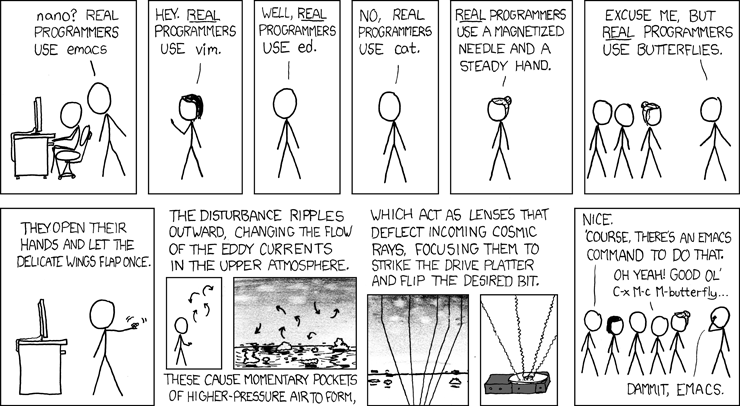
\includegraphics[scale=0.6]{images/real_programmers.png}
\end{center}

\section{How to get credit for this Skill Module}
There are 4 steps to completing this Skill Module.
\begin{enumerate}
\item Read this document
\item Run \texttt{vimtutor} and complete it
\item Use vim for a while on your own
\item Complete the questions and return them to your UGTA
\end{enumerate}

\noindent
Your finished product should have the following things:
\begin{itemize}
\item A brief description of your experience with vim.
\item The questions answered to your best ability
\end{itemize}

\section{Introduction}
Vim is a text editor written in $1988$ by Bram Moolenar, now an
employee at Google. Vim stands for {\em Vi IMproved} as it is based
on the older text editor Vi, but is thought to have a feature set
that surpasses that of Vi. It now comes default on basically any
linux distribution you could possibly imagine using, and has become
extremely popular in the Unix community since its onset. 

\subsection{Why Learn Vim?}
With powerful IDEs like Eclipse and Netbeans available, you might ask why
its even worth learning vim. While to some extent vim does not contain
all the features that these IDEs contain, vim is still an 
extremely powerful text editor that will make you much more efficient.
It has an extremely rich set of functionality that will allow you to 
edit text in ways that conventional text editors do not allow. Also,
vim is extremely lightweight and there will be many times when you
do not need a powerful IDE, or cannot even use one. It's one of those
things that once you start using, you will begin to appreciate.

And bottom line, if you are a computer science major then you will {\bf need}
to learn how to use a unix text editor. You'll be forced more and more
to work in terminal environments where getting a graphical interface is not
really possible, and your efficiency in coding will be highly dependent
upon your ability to use a text editor effectively.

\section{Getting Vim}
Vim is available for all operating systems and architectures, and I will
outline how you can get a hold of it on different systems. However, 
{\bf I highly recommend you work on a linux system. Most of the skill module 
assumes you are in a Linux environment, and some parts even require it.}

If you do not have linux installed on your computer, or you find it troubling
to installing it, you can always use the CS machines in ENS basement or 
in PAI.

\subsection{Linux}
If you want to install in a linux environment, obtain vim from your package 
manager. For instance, on Ubuntu you would do:
$$\text{\texttt{sudo apt-get install vim}}$$
You can also obtain the graphical version of vim by doing (this package
contains both the normal version and the graphical version):
$$\text{\texttt{sudo apt-get install vim-gnome}}$$

\subsection{Windows}
Follow this link to obtain \texttt{Gvim}. \texttt{Gvim} is a graphical
version of vim:
\url{http://www.vim.org/download.php#pc}

\subsection{Mac}
Consult the following link. \url{http://www.vim.org/download.php#mac}.

\section{Understanding Vim Configuration Files}
{\bf Note: this only applies if you develop on a *nix environment.}

As a consequence of vim's rich functionality, vim is 
extremely configurable. You can change how it behaves with regards to 
colorschemes, syntax coloring, tab spacing, highlighting, etc. 
To deal with all of this, Vim uses a \emph{configuration file} named 
\texttt{.vimrc}. On linux systems, files whose names are prefixed by dots 
are hidden. This means that when running \texttt{ls}
or just looking through your file explorer, they will not be shown by default.
(As an aside, to view hidden files when in terminal run
\texttt{ls -a}, the \texttt{-a} standing for 'all'.)

Vim knows where to look for this configuration file. The location 
it looks first is in your home directory, i.e. \texttt{\textasciitilde/.vimrc}. I won't
go into detail here about actually writing your own configuration files;
for now, copy mine and as you use vim more you can change it suit
your own purposes. I've included the file on the website. 
Download the file and place it in your home directory after you install vim.
{\em Ensure that the filename is .vimrc, not anything else like .vimrc.txt}.

\section{Editing in Vim}
It's finally time to begin learning to use vim!

If you have already tried opening vim and editing a file, you may have
noticed that it's not exactly intuitive. In fact, without any previous
knowledge of vim it is probably impossible to edit a file. 
However, there aren't a lot of things you need to learn to become
relatively efficient in vim. 

There are two modes in vim, {\bf Command Mode} and {\bf Insert Mode}.
{\bf Insert Mode} is what you'd expect; you can type normally just
like any other text editor. {\bf Command Mode}, or the mode in which
Vim normally begins, is the mode where you can run different commands
to edit the text. 

\subsection{Insert Mode}
Insert Mode is just like being in notepad. You can type text, delete
text, etc. There's not much to it. 

\subsection{Command Mode}
Command Mode is where vim's true usefulness shows. From command mode, you can run
different commands, or basically keyboard shortcuts, to manipulate and traverse
text. For instance when in Command Mode, pressing 'w' will move your cursor
to the next word, pressing 'gg' will take your cursor to the top of the file,
pressing 'dd' will delete the current line, pressing 'p' will paste the last
thing in the buffer, etc. etc. This list goes on and on, and in the next section
we'll tackle learning a useful subset of this list.

\subsection{Switching Between Modes}
This all begs the question, how does one get to either mode? By default, Vim
starts you out in Command Mode. To get to insert mode, press 'i'. To get out of
insert mode and back to command mode, press '$\langle$ESC$\rangle$'. And it's that easy.

\section{\texttt{vimtutor}}
So there already exist many tools for learning to use Vim. One among them is called
\texttt{vimtutor}. This program can be obtained from your package manager in Linux,
and is also on the CS machines.

To run this program, open up a terminal and run the command \texttt{vimtutor}.
After that, just follow along. It's honestly not that long, and is very
helpful in learning how to use Vim properly. Note that vimtutor is really nothing
more than editing a text file in vim. 

\section{Conclusion}
As I hope you will come to see, Vim is an extremely powerful text editor that
despite its age has still maintained vast popularity in the development
community. {\bf If you read nothing else in this entire Skill Module, please
at least read this. The only way to really learn Vim is to go out and use it.
It will be annoying to use initially, and you will feel less efficient. However
this 'breaking-in' period will be short, and as you become more proficient
you will come to appreciate Vim's many features in editing text.}

{\bf The only way to get better at Vim is to constantly question how you do 
things. Do not get set in habits, but rather catch yourself 
and always question if there is a faster way to do what you are doing.}

\section{Advanced Vim}
There are more advanced features of vim that \texttt{vimtutor} did not cover,
and I will not cover here. However, I encourage you to go out on your own time
and learn about these things as you become more familiar with vim. Here's
a list of things that I think you may find interesting to learn more about:
\begin{itemize}
\item Vim Plugins and Colorschemes
\item Markers
\item Registers
\item Macros
\item Window Splits
\item Vimdiff
\item Fixing Code Indentation
\item Code Complete (Yes, Eclipse-style)
\end{itemize}

\noindent
And there's much more that I don't even know about!

\section{Questions}

\begin{figure}
\begin{center}
\leavevmode
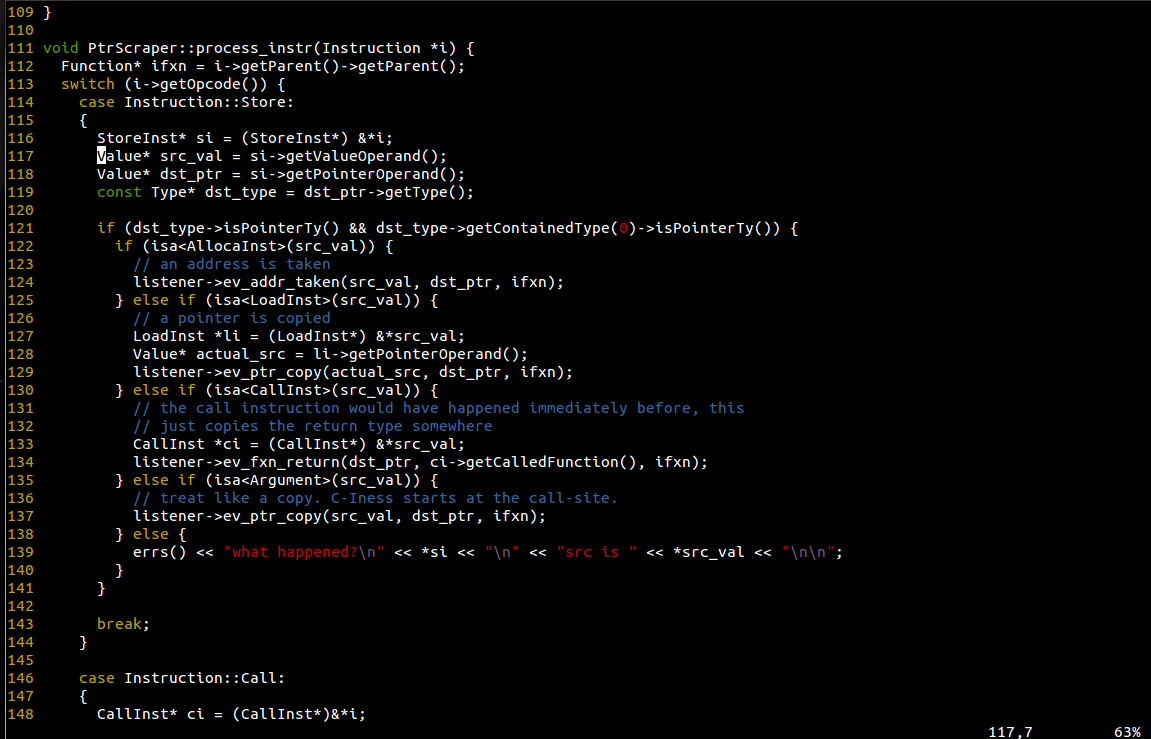
\includegraphics[scale=0.3]{images/question-pic.png}
\end{center}
\caption{Code Snippet}
\label{fig:questionpic}
\end{figure}

Consider Figure \ref{fig:questionpic}. Each question will ask you to take some
action upon the text, and answer as if your cursor is in the current position.
{\bf Pick $12$ of the $20$ and answer them.} 
\\\\
In {\bf bold} next to every question, i've indicated how many characters
it took me to do it. This is not suggesting that you should get the same number,
or that I've achieved the best way to do it. It is just a guide to help you
think in the right direction, and you won't be penalized for not getting it
in the exact same way. Just try your best.

\begin{enumerate}
\item This is a gimme. Describe how to move left, right, up and down from the keyboard.
\item How do you undo a change? Redo? ({\bf 1})
\item How can you delete the whole line? ({\bf 2})
\item How can you delete the current line and the next 5? ({\bf 3})
\item How can you duplicate the current line in place? ({\bf 3})
\item How can you bring your cursor to sit upon the equal sign? ({\bf 3 })
\item For this question assume your cursor is at the equal sign. Now delete the rest of the line. ({\bf 2})
\item Same context as previous question. Delete until beginning of the line ({\bf 2})
\item How can you delete only the word 'Value' upon which the cursor sits? ({\bf 2})
\item Page Up? Page Down? (Don't hit the page-up key). ({\bf 2 for each})
\item How can you jump backward by words? ({\bf 1})
\item How can you get to the beginning/end of the line? Of the file? ({\bf 2, 1})
\item Delete the contents of the entire file. ({\bf 4})
\item Find the matching end-brace of the brace on line $115$. {\bf 3}
\item Delete everything contained from the brace on line $115$ to its match. ({\bf 4})
\item Search for all instances of \texttt{src\_val}. ({\bf Theres really only one way to do the search and replace ones, and the length isn't important})
\item Replace \texttt{src\_val} with \texttt{sv}. 
\item Now modify that to work for any number of instances on the line.
\item Now modify that to work for the entire program.
\item Now modify that to prompt you before making changes.

\end{enumerate}

\section{Contact}
If at any point you have questions about this Skill Module, Vim, or anything
in general, do not in the slightest hesitate to email me at 
\url{parth.upadhyay@gmail.com}. I would be more than happy to help you out.
Also feel free to forward me suggestions/thoughts you have about this skill module.
\\\\
You can freely get a copy of the source of the skill module here:
\url{https://github.com/parthupadhyay/Vim-Skill-Module}.
\end{document}
